\section{Durchführung}
\label{sec:Durchführung}

\subsection{Aufbau und Funktionen der Apparatur}
\label{sec:d1}
Der Plan der aller Komponenten und deren Installation befindet sich in \autoref{fig:d1}.
Der blau markierte Bereich grenzt die Komponenten ein, die zu dem Abhörere Eve 
gehören, sie kann nach Belieben in das Experiment eingebunden werden. Der reale 
Aufbau ist in \autoref{fig:d2} zu sehen.
\begin{figure}[H]
    \centering
        \centering
        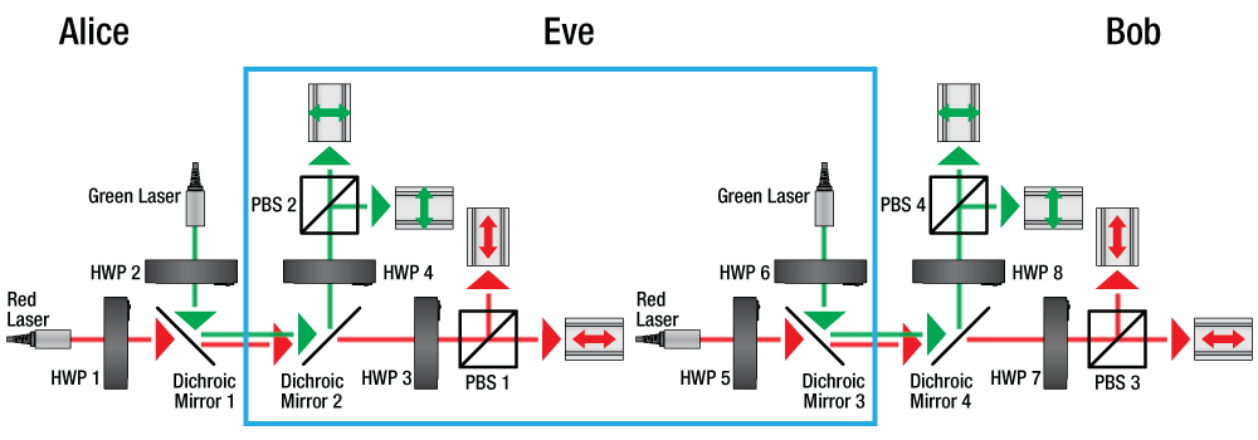
\includegraphics[width=0.95\textwidth]{Bilder/schema.png}
        \caption{Alle Optikmodule und deren Verknüpfungen. HWP steht für 
        Half-Wave Plate, um das Licht zu polarisieren. PBS steht für 
        Polarization Beam Splitter und teilt das Licht. \cite{anleitung14}}
    \hfill
    \label{fig:d1}
\end{figure}
\begin{figure}[H]
    \centering
        \centering
        
\includegraphics[width=0.95\textwidth]{Bilder/aufbau.jpg}
        \caption{Bild der Apparatur. (Eigenaufnahme)}
    \hfill
    \label{fig:d2}
\end{figure}
\noindent Alice verfügt als Sender über zwei Laserquellen unterschiedlicher Wellenlängen,
davor befinden sich jeweils die Polarisationsfilter, mit denen die
Polarisationszustände der einzelnen Pulse eingestellt werden. Über einen
Strahlteiler werden die Pulse in die gemeinsame Übertragungsstrecke eingespeist. 
Bob als Empfänger verfügt hinter seinen Filtern für jede Wellenlänge über zwei Detektoren,
sodass er entweder Einsen oder Nullen empfangen kann. Eve als Abhörer ist zunächst 
mit gleichen Komponenten wie Bob ausgestattet, um die Photonen zu messen. Für die
Weiterleitung an Bob ist das Modul darüber hinaus mit einer Sendeeinheit analog zu
Alice . 
\\
\noindent Bevor die Messungen gestartet werden, müssen alle Komponenten korrekt 
aufeinander justiert sein. Um das zu überprüfen, werden die Einstellungen aus 
\autoref{fig:d3} übernommen und kontrolliert, ob die Bit-Ausgaben mit den Erwartungen 
zusammenpassen.
\begin{figure}[H]
    \centering
        \centering
        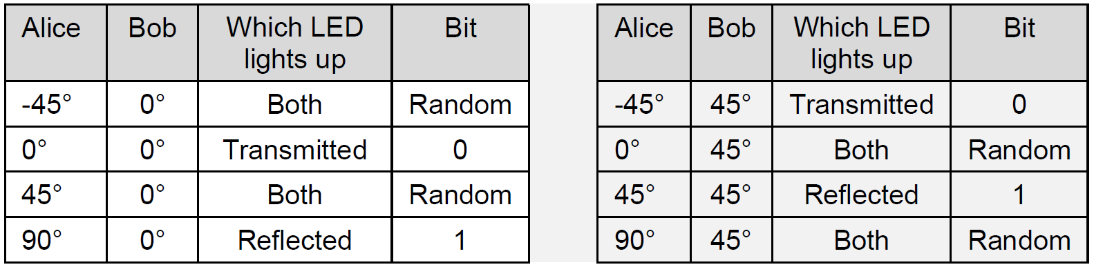
\includegraphics[width=0.95\textwidth]{Bilder/jprüf.png}
        \caption{Einstellungen zum Prüfen der Justierung. \cite{anleitung14}}
    \hfill
    \label{fig:d3}
\end{figure}

\subsection{Standard BB84}
Nach Überprüfen der Justage beginnt der Versuchsteil mit der Raw Key Generierung.
Von Alice werden 52 zufallsgenerierte Signale über den roten Laser gesendet. Für
jedes Bit wird eine der beiden Basen genutzt:
\begin{itemize}
    \item \textbf{Geradlinige Basis +:} Polarisation 0° für Bit 0 und 90° für Bit 1
    \item \textbf{Diagonale Basis $\times$:} Polarisation -45° für Bit 0 und +45° für Bit 1
\end{itemize}
Bob empfängt die Signale von Alice, ebenfalls in einer willkürlichen Basis. Nach
der Datenübermittlung wird die Sifting Phase eingeleitet, hier wird überprüft,
welche Daten von Alice und Bob übereinstimmen. Alle Werte, wo Basis und Bit nicht
identisch sind, werden verworfen.
\\
\noindent Als nächstes wird das Modul Eve gemäß der Markierung in \autoref{fig:d1}
zwischen Alice und Bob in den Strahlengang eingefügt. Nach der mechanischen 
Installation werden erneut die acht Testpolarisationen aus \autoref{fig:d3}
überprüft, um sicherzustellen, dass Eves Detektion und ihre Weiterleitung an Bob
korrekt funktionieren. Das Messverfahren funktioniert so wie zuvor: Von Alice werden 
52 Bits in einer zufälligen Basis gesendet. Bei Eve werden die Pulse abgefangen 
und in einer zufälligen Basis gemessen. Der neue Puls wird in der entsprechenden 
Basis an Bob gesendet, wo (wie zuvor) der Puls empfangen und gemessen wird. 
Nach der Übertragung aller Pulse wird für Alice und Bob ein Basisabgleich 
durchgeführt und die Fehlerrate bestimmt. 

\subsection{BB84 mit decoy states}
Die Messung mit decoy states wird analog zum Standard BB84 durchgeführt, allerdings
enthalten die Pulse von Alice nicht nur Signale vom roten Laser, sondern auch vom 
grünen Laser. Nach der Übertragung und dem Abgleich wird wieder Eve eingebunden.
Es werden erneut 52 zufällig generierte Signale von dem Alice Modul gesendet 
und bei Eve abgefangen. Das gemessene Signal wird an Bob weitergeleitet und 
dort gemessen.